\subsection{Surface Oscillations}

Oscillations in surface radius at $\sim 10 \mathrm{yr}$ to core collapse were also observed, increasing in amplitude before dying away. Notably, they only feature in high resolution models, where low resolution models show more erratic changes in radius (see Figure \ref{fig:Comparing-Radii}). 

%As noted in Section \ref{sec:Method}, the resolution was also altered, providing interesting comparisons. Notably, only with high-resolution models are oscillations, as seen in Figure \ref{fig:Comparing-Radii} (an example of such an event seen in Figure \ref{fig:KHD_Compare_Metal}), where only the high resolution models show this regular oscillatory change in radius with time (independent of mixing theory).

%This is further illustrated in Figure \ref{fig:KHD_Compare_Metal}, where a

The magnitude of such oscillations do, however, vary dramatically. Figure \ref{fig:KHD_Compare_Metal} shows how the \gls{SolarMetal} model clearly shows this oscillatory pattern, expressed throughout the envelope, whilst the \gls{LowMetal} model expresses this at scales too small for the diagram. 

The cause is likely numerical, owing to how surface oscillations are expected during phases of instability, such as during the red supergiant phase, but they were not possible to accurately recreate with the model used (see Section \ref{sec:TDC}). 

%add a reference??
%write a little more explainig this?

%\begin{figure*}[t]
\begin{center}
    \includegraphics[width=0.7\linewidth]{Figures/KHD_Compare_Metal.pdf}
    \caption{Kippenhahn diagrams of radius (logarithmic) by time until core collapse, comparing a \gls{LowMetal} (lower) and \gls{SolarMetal} (upper) run using \gls{MLT} and short timestepping. Colour pertains to Mach number and label locations are based off of \citealp{Polls11}.}
    \label{fig:KHD_Compare_Metal}
\end{center}
\end{figure*}
\begin{figure}[H]
\begin{center}
    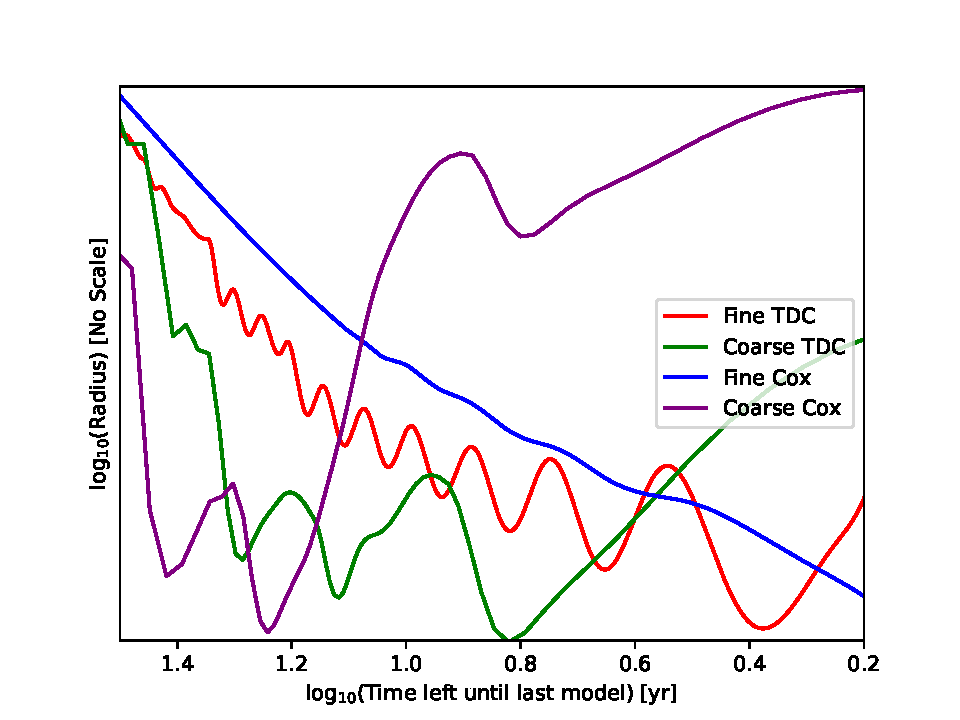
\includegraphics[width=0.8\linewidth]{Figures/Comparing-Radii.pdf}
    \caption{Relative change in stellar radius in four models, varying only by mixing theory and resolution (Fine = high resolution, Coarse = test run resolution).}
    \label{fig:Comparing-Radii}
\end{center}
\end{figure}